\documentclass{scrartcl}

\include{header/zusammenfassung}
\usepackage{tikz}
\usetikzlibrary{shapes}
\usepackage{adjustbox}
\usepackage{multicol}
\usetikzlibrary{arrows}
\usetikzlibrary{calc}
\usepackage{booktabs}
\usepackage{tabularx}
\usepackage{siunitx}
\sisetup{detect-all,per-mode=symbol}
\usepackage{pdfpages}
\usepackage[version=3]{mhchem}

\title{FTP\_Physics}
\subtitle{The Physics of Materials and Engineering Devices}
\author{H.Badertscher}

\begin{document}
\selectlanguage{english}
\numberwithin{equation}{section}
\numberwithin{table}{section}
\numberwithin{figure}{section}

\maketitle

\section{Definitions}

\begin{tabularx}{\linewidth}{Xlll}

	Planck's constant & $h$ & $6.626 \cdot 10^{-34}$ & \si{\J\second} \\
		& $\hbar$ & $h / 2\pi$ & \\
	Mass of an electron & $m_e$ &  $9.109 \cdot 10^{-31}$ & \si{\kilogram} \\
	Charge of an electron & $q_e$ & $1.6 \cdot 10^{-19}$ & \si{\coulomb} \\
	Absolute permeability & $\varepsilon_0$ & $8.85 \cdot 10^{-12}$ & \si{\ampere\second\per\volt\per\meter} \\
	Avogadro constant  ($\stackrel{\wedge}{=}1$\si{\mol})& $N_A$ & $6.0221 \cdot 10^{23}$ & \\
	Boltzmann constant $k_B = R / N_A$& $k_B$ & $1.381 \cdot10^{-23}$ & \si{\J\per\K} \\
	Ideal gas constant & $R$ & $8.314$ & \si{\J\per\mol\per\K} \\
	Electron volt & $e$ & $1$ & \si{\eV} \\
		& & $1.6 \cdot 10^{-19}$ & \si{\J} \\ 
	Speed of light & $c$ & $299'792'458$ & \si{\meter\per\second} \\
\end{tabularx}

\subsection{Percentages}
Weight percents (wt\%) are the fraction of the weight, while atomic percents (at\%) are the fraction of the number of atoms.
\section{Basic concepts}

Schroedinger Equation
\begin{equation}
	i \hbar \frac{\partial\Psi(x,t)}{\partial t} = U(x) \cdot \Psi(x,t) - \frac{\hbar}{2m} \frac{\partial^2 \Psi(x,t)}{\partial x^2}
\end{equation}

%TODO: beschreiben
\begin{equation}
	L_n = r m_e v = n \frac{h}{2\pi} = n \hbar \qquad n = 1,2,3,\dots
\end{equation}

%TODO: weitere gleichungen

Bohr radius
\begin{equation}
	r_0 = a_0 = \frac{\varepsilon_0 h^2}{\pi m_e q_e^2}
\end{equation}

\subsection{Mean kinetic energy and temperature}
Ideal gas equation
\begin{equation}
	PV = \frac{1}{3} Nm \cdot \bar{v^2} = \frac{N}{N_A}RT = N k_B T
\end{equation}

Average kinetic energy per molecule
\begin{equation}
	E_{kin} = \frac{1}{2} m \bar{v^2} = \frac{3}{2} k_B T
\end{equation}

Gas pressure in the kinetic theory
\begin{equation}
	P = \frac{1}{3} \rho \bar{v^2}
\end{equation}

Root mean square velocity
\begin{equation}
	v_{rms} = \sqrt{\frac{3 k_B T}{m}} = \sqrt{\frac{3RT}{M}}
\end{equation}

\subsection{Electric Noise}
Root mean square voltage
\begin{equation}
	v_{rms}  = \sqrt{4 k_B T R B}
\end{equation}
where $B$ is the Bandwith of the $RC$ network.

\subsection{Molecular velocity and energy distribution}
Velocity distribution function
\begin{equation}
	n_v = N \cdot 4 \pi \left(\frac{m}{2\pi k_B T}\right)^2 v^2 e^{-\left(\frac{m v^2}{2 k_B T}\right)}
\end{equation}

Boltzmann factor
\begin{align}
	e^{-\left(\frac{E}{k_B T}\right)} \\
	\frac{n_E}{N} = C_E \cdot e^{-\left(\frac{E}{k_B T}\right)}
\end{align}

\subsection{Energy of a photon}

\begin{equation}
	E = h \cdot f = \hbar \cdot \omega = \frac{h \cdot c}{\lambda}
\end{equation}

Where the wave length $\lambda = \frac{c}{f}$. 
% !TeX spellcheck = en_US
\section{Molecular bonding}
The two principal types of bonds are the ionic and the covalent bond. 
Other types of bonds are van der Waals bonds, metallic bonds and hydrogen bonds.

Balance between attractive force $E_A$ (e.g. Coulomb force) and repulsive force $E_R$ (shell overlap).

\begin{figure}[ht]
    \centering
    \begin{tikzpicture}
\pgfplotsset{ticks=none}
\pgfplotsset{every axis x label/.style={
    at={(0.5,0)},
    below,
    yshift=-5pt}
}
\pgfplotsset{every axis y label/.style={
    at={(0,0.5)},
    xshift=-15pt,
    rotate=90}
}

\begin{scope}[shift={(-5,0)}]
    \begin{axis}[domain=0.05:1,samples=101,
        width = 8cm, height = 6cm,
        xlabel={Interatomic separation $r$},
        ylabel={Force},
        xmin = 0.1, xmax = 0.5,
        ymin = -1000, ymax = 1000,
    ]
        \addplot[black!80,mark=none] coordinates {(0,0)(1,0)};
        \node at (axis cs:0.11,65) {0};
        \addplot[HSRBlue,mark=none] {20/(x^2)};
        \addplot[HSRBlue,mark=none] {-0.25/(x+0.1)^6};
        \addplot[HSRHematite,mark=none] {20/(x^2) - 0.25/(x+0.1)^6};
        \node[label={$r_0$},circle,fill=HSRHematite,inner sep=2pt] at (axis cs:0.16334,1) {};
        \node at (axis cs:0.25,500) {$F_A$};
        \node at (axis cs:0.21,-500) {$F_R$};
        \node at (axis cs:0.25,65) {$F_N$};
    \end{axis}
\end{scope}

\begin{scope}[shift={(+5,0)}]
    \begin{axis}[domain=0:1,samples=101,
        width = 8cm, height = 6cm,
        xlabel={Interatomic separation $r$},
        ylabel={Potential Energy},
        xmin = 0, xmax = 0.8,
        ymin = -200, ymax = 100,
    ]
        \addplot[black!80,mark=none] coordinates {(0,0)(1,0)};
        \node at (axis cs:0.02,15) {0};
        \addplot[HSRBlue,mark=none] {-20/x};
        \addplot[domain=0.11:1,HSRBlue,mark=none] {1/(20*(x+0.1)^5)};
        \addplot[HSRHematite,mark=none] {1/(20*(x+0.1)^5) - 20/x};
        \node[label={ $r_0$},circle,fill=HSRHematite,inner sep=2pt] at (axis cs:0.16334,-82.96) {};
        \node at (axis cs:0.4,20) {$E_R$};
        \node at (axis cs:0.4,-70) {$E_A$};
        \node at (axis cs:0.4,-30) {$E$};
    \end{axis}
\end{scope}


\end{tikzpicture}
    \caption{Force and energy in molecular bonding}
\end{figure}

where $r_0$ is the equilibrium separation and $E_0$ the bond energy at equilibrium.

\subsection{Ionic bonding}
%TODO: add images / example

\begin{equation}
	E(r) = -\frac{e^2 M}{\varepsilon_0 4 \pi r} + \frac{B}{r^m}
\end{equation}
where $M$, $B$ and $m$ are constants. 

$M$ is the Mandelung constant, which models Coulomb interactions in the ionic crystal.
It depends on the crystal type and is $M=1.748$ for a \ce{NaCl} type (FCC).
For NaCl crystal, $B=\SI{6.972e-96}{\joule\meter\tothe{8}}$ and $m=8$.

\subsection{Covalent bonding} 
Atoms share electrons to fill their valence bands.

\subsection{Metallic bonding}
Atoms are held together by electron gas.

\subsection{Secondary (Van der Waals) bonding}
Weak force between polar molecules (dipoles, e.g. \ce{H2O}). 

\subsection{Comparison} ~\\
\begin{table}[ht]
    \begin{tabularx}{\linewidth}{p{2cm}p{1.5cm}p{1.4cm}p{1.4cm}p{1.5cm}lX}
    	& Typical Solids & Bond Energy  & Melt. Temp. & Elastic Modulus & Density & Typical Properties \\ \toprule
    	Ionic & NaCl & 3.2 & 801 & 40 & 2.17 & El. insulators (may become conductive at high temperatures). \\
    	 & MgO & 10 & 2852 & 250 & 3.58 & High elastic modulus. Hard and brittle but cleavable. Th. conductivity less than metals.\\
    	Metallic & Cu & 3.1 & 1083 & 120 & 8.96 & El. conductor. \\
    	 & Mg & 1.1 & 650 & 44 & 1.74 & Good th. conduction. High elastic modulus. Generally ductile, can be shaped. \\
    	Covalent & Si & 4 & 1410 & 190 & 2.33 & Large elastic modulus, hard and brittle. \\
    	  & C & 7.4 & 3550 & 827 & 3.52 & Diamond. Hardest material, good el. insulator. \\
    	van der Waals: Hydrogen & PVC & - & 212 & 4 & 1.3 & Low elastic modulus. Some ductility \\
    	 & H$_2$O (ice) & 0.52 & 0 & 9.1 & 0.917 & El. insulator, poor th. conductivity, large thermal expansion. \\
        van der Waals: Induced dipole & Crystalline Argon & 0.09 & -189 & 8 & 1.8 & Low elastic modulus, el. insulator, poor th. conductivity, large th. expansion. \\
    	\bottomrule
    \end{tabularx}
    \caption{Comparison of bond types and typical properties}
\end{table}

\subsection{Crystal structures}

The atomic packaging factor $\mathrm{APF}$ is defined as
\begin{equation}
    \mathrm{APF} = \frac{\text{Volume of atoms in unit cell}}{\text{Volume of unit cell}}
\end{equation}

\begin{figure}[ht!]
    \centering
    \begin{subfigure}[t]{0.32\linewidth}
        \centering
        \includegraphics[width=0.9\textwidth]{images/fcc.png}
        \caption{Face-centered cubic (FCC)}
    \end{subfigure}
    \begin{subfigure}[t]{0.32\linewidth}
        \centering
        \includegraphics[width=0.9\textwidth]{images/bcc.png}
        \caption{Body-centered cubic (BCC)}
    \end{subfigure}
    \begin{subfigure}[t]{0.32\linewidth}
        \centering
        \includegraphics[width=0.9\textwidth]{images/hcp.png}
        \caption{Hexagonal close-packed (HCP)}
    \end{subfigure} 
    
    \begin{subfigure}[t]{0.24\linewidth}
        \centering
        \includegraphics[width=0.9\textwidth]{images/diamond.png}
        \caption{Diamond unit cell}
    \end{subfigure}
    \begin{subfigure}[t]{0.24\linewidth}
        \centering
        \includegraphics[width=0.9\textwidth]{images/zns.png}
        \caption{Zinc blende (ZnS) cubic structure}
    \end{subfigure} 
    \begin{subfigure}[t]{0.24\linewidth}
        \centering
        \includegraphics[width=0.9\textwidth]{images/nacl.png}
        \caption{Ionic NaCl crystal structure}
    \end{subfigure}  
    \begin{subfigure}[t]{0.24\linewidth}
        \centering
        \includegraphics[width=0.9\textwidth]{images/cscl.png}
        \caption{Ionic CsCl crystal structure}
    \end{subfigure}     
    \caption{Comparison of unit cells}
\end{figure}

\begin{table}[ht!]
    \centering
    \begin{tabularx}{0.9\linewidth}{p{2cm}p{2cm}p{2.5cm}p{1.8cm}p{1.5cm}X}
    \toprule
        Crystal Structure & $a$ and $R$ & Coordination Number (CN) & Atoms per unit cell & APF & Examples \\ \midrule
        Simple cubic & $a = 2R$ & 6 & 1 & 0.52 & None \\
        BCC & $a=4R/\sqrt{3}$ & 8 & 2 & 0.68 & Metals: $\alpha-$Fe, Cr,Mo,W \\
        FCC & $a=4R/\sqrt{2}$ & 12 & 4 & 0.74 & Metals: Ag, Au, Cu, Pt \\
        HCP & $a=2R$, $c=1.633a$ & 12 & 2 & 0.74 & Metals: Co, Mg, Ti, Zn \\
        Diamond & $a=8R/\sqrt{3}$ & 4 & 8 & 0.34 & Covalent solids: Diamond, Ge, Si, $\alpha-$Sn \\
        ZnS & & 4 & 8 & 0.34 & Covalent and ionic solids, compound semiconductors: ZnS, GaAs, GaSb, InAs, InSb \\
        NaCl & & 6 & 4 cations, 4 anions & 0.67 & Ionic solids: NaCl, AgCl, LiF, MgO, CaO \\
        CsCl & & 8 & 1 cation, \newline 1 anion & & Ionic solids: CsCl, CsBr, CsI \\
    \bottomrule
    \end{tabularx}
    \caption{Properties of some important crystal structures}
\end{table}

\subsection{Allotropy and carbon}
Certain substances can have more than one crystal structure. 
E.g. carbon has eight allotropes: Diamond, Graphite, Lonsdaleite, $C_{60}$ (buckyball), $C_{540}$, $C_{70}$, amorphous carbon and single-walled carbon nanotube.
\section{Electric conduction}

Ohm's law for the electric current density $J$ is
\begin{equation}
    J = \sigma E = e n v_d
\end{equation}
with the drift velocity
\begin{equation}
    v_d = \frac{e \tau}{m_e} E = \mu_d E \quad \approx \SI{1e-4}{\meter\per\second}
\end{equation}
and drift mobility being
\begin{equation}
    \mu_d = \frac{e \tau}{m_e} = \frac{e l}{m_e u}
\end{equation}
Conductivity
\begin{equation}
    \frac{1}{\rho} = \sigma = e n \mu_d = \frac{e^2 n \tau}{m_e} = \frac{e^2 n l}{m_e u}
\end{equation}
With the relaxation time
\begin{equation}
    \tau = \frac{1}{\pi a^2 u N_s}
\end{equation}
The mean free path length is
\begin{equation}
    l = u \tau
\end{equation}

Matthiessen's rule
\begin{equation}
    \rho = \rho_0 \left[ 1 + \alpha_0 \left( T - T_0 \right) \right]
\end{equation}

% !TeX spellcheck = en_US
\section{Quantum physics\buch{191}}

A photon has the energy
\begin{equation}
    E_{ph} = h v
\end{equation}

The electron wavelength is found to be
\begin{equation}
    \lambda = \frac{h}{p} = \frac{c}{v}
\end{equation}
where $h$ is the Planck's constant.

The electron momentum is 
\begin{equation}
    p = m v
\end{equation}

\begin{table}[ht!]
    \centering
    \begin{tabular}{lll}
        & Photon & Electron \\ \toprule
        Energy & $E = h \nu = \hbar \omega$ & $E = \hbar \omega = \frac{p^2}{2m}$ \\
        Momentum & $p = \frac{h}{\lambda} = \hbar k$ & $p = \frac{h}{\lambda} = \hbar k = m \nu$ \\ \bottomrule
    \end{tabular} \\
     with $\hbar = \frac{h}{2\pi}$ and $k = \frac{2\pi}{\lambda}$
\end{table}

\subsection{Schrödinger Equation\buch{208}}
The wave function of a free electron is
\begin{equation}
    \Psi(x,t) \,\propto\, e^{i (kx-\omega t)}
\end{equation}
The Schrödinger equation for motion of a particle of mass $m$ in potential $V(x,t)$ is then
\begin{equation}
    i \hbar \frac{\partial}{\partial t} \Psi = - \frac{\hbar^2}{2m}\frac{\partial^2}{\partial x^2} \Psi + V(x,t) \Psi
\end{equation}
eliminating time dependence leads to the time-independent Schrödinger equation for $V=V(x)$
\begin{equation}
    \frac{d^2 \varPsi}{d x^2} + \frac{2m}{\hbar^2}(E-V) \varPsi = 0
\end{equation}
one can get the time-dependent wave function $\Psi$ from the time-independent wave function $\varPsi$ by
\begin{equation}
    \Psi(x,t) = \varPsi(x) e^{-i \omega t}
\end{equation}
where $\omega = \frac{E}{\hbar}$.

\subsection{Infinite Potential Well\buch{212}}
\begin{figure}[ht!]
    \centering
    \begin{tikzpicture}
\begin{scope}[shift={(-5,0)}]
    \begin{axis}[ticks=none, axis lines=middle, clip=false,
    xmin=0,xmax=6,ymin=0,ymax=1.2,
    width=8cm,height=4cm,
    xlabel={x},ylabel={V(x)},
    every axis x label/.style={
        at={(ticklabel* cs:1)},
        anchor=west,
    },
    every axis y label/.style={
        at={(ticklabel* cs:1)},
        anchor=south,
    },
    ]
        \addplot[mark=none] coordinates {
            (0,1)
            (2,1)
            (2,0)
            (4,0)
            (4,1)
            (6,1)
        };
        
        \node[anchor=north] at (xticklabel cs:0.333) {0};
        \node[anchor=north] at (xticklabel cs:0.666) {a};
        \node[anchor=east] at (yticklabel cs:0) {0};
        \node[anchor=east] at (yticklabel cs:0.833) {$\infty$};
        
        \node[label={Electron},draw=HSRBlue,fill=HSRBlue60,circle,minimum size=0.2] at (axis cs:2.8,0.4){};
    \end{axis}
\end{scope}
\begin{scope}[shift={(+5,0)}]
    \begin{axis}[ticks=none, axis lines=middle, clip=false,
    width=6cm,height=4cm,
    domain=0:1,
    samples=101,
    ymin=0, ymax=7,
    ]
        \addplot[HSRBlue,mark=none] {sin(deg(1*pi*x))};
        \addplot[HSRBlue,mark=none] {2+sin(deg(2*pi*x))};
        \addplot[HSRBlue,mark=none] {4+sin(deg(3*pi*x))};
        \addplot[HSRBlue,mark=none] {6+sin(deg(4*pi*x))};
        \node[anchor=north] at (xticklabel cs:0) {0};
        \node[anchor=north] at (xticklabel cs:1) {a};
        \node[anchor=east] at (yticklabel cs:0.142) {$\Psi_1$};
        \node[anchor=east] at (yticklabel cs:0.380) {$\Psi_2$};
        \node[anchor=east] at (yticklabel cs:0.618) {$\Psi_3$};
        \node[anchor=east] at (yticklabel cs:0.857) {$\Psi_4$};
    \end{axis}
\end{scope}
\end{tikzpicture}
    \caption{Infinite potential well}
\end{figure}
The boundary conditions $\Psi=0$ for $x\leq 0$ and $x\geq a$ lead to the Schrödinger equation
\begin{equation}
    \frac{d^2 \Psi}{d x^2} + \frac{2m}{\hbar^2} E \Psi = 0
\end{equation}
Which leads to a wave function $\Psi(x) \propto \sin kx$ with $ka=n\pi$ for $n=1,2,\ldots$, i.e. $\Psi_n(x) \propto \sin\frac{n\pi}{a}x$
The energy is thus
\begin{equation}
    E_n = \frac{h^2 n^2}{8 m a^2}
\end{equation}
where $E_1$ is the ground energy.

\subsection{Tunneling\buch{221}}
\begin{figure}[ht!]
    \centering
    \begin{tikzpicture}[scale=0.6]
    % Border
    \draw[thick] (0,0) -- (2,0) -- (2,4) -- (4,4) -- (4,0) -- (6,0);
    
    % Sine waves
    \draw[HSRBlue] (0,2.5) sin (0.25,3.0) cos (0.5,2.5) sin (0.75,2.0) cos (1,2.5) sin (1.25,3.0) cos (1.5,2.5) sin (1.75,2.0) cos (2,2.5);
    \draw[HSRBlue] (2,2.5) to[out=290,in=170] (4,1.5);
    \draw[HSRBlue] (4,1.5) sin (4.25,1.75) cos (4.5,1.5) sin (4.75,1.25) cos (5,1.5) sin (5.25,1.75) cos (5.5,1.5) sin (5.75,1.25) cos (6,1.5);
    
    % Text
    \node at (1,0.5) {\tiny Sine wave};
    \node at (3,0.5) {\tiny Exp. decay};
    \node at (5,0.5) {\tiny Sine wave};
    
\end{tikzpicture}
    \caption{Electron tunneling}
\end{figure}

The Schrödinger equation becomes
\begin{equation}
    \frac{d^2 \Psi}{dx^2} + \begin{Bmatrix} k^2 \\ -\alpha^2 \end{Bmatrix} \Psi = 0
\end{equation}
with
\begin{equation}
    \left.\begin{matrix}
        k^2 &= \frac{2m}{\hbar^2} (E-V_{I,III}) \\
        \alpha^2 &= \frac{2m}{\hbar^2}(V_{II}-E)
    \end{matrix}\right\}
    \quad\text{for}\quad
    \left\{\begin{matrix}
        E>V_{I,III}=0\\
        E<V_{II}=V_0
    \end{matrix}\right.
\end{equation}

The wave functions in the 3 regions are
\begin{align}
    \Psi_{I}(x) &= A_1 e^{ikx} + A_2 e^{-ikx} \\
    \Psi_{II}(x) &= B_1 e^{\alpha x} + B_2 e^{-\alpha x} \\
    \Psi_{III}(x) &= C_1 e^{ikx} + C_2 e^{-ikx} 
\end{align}
Applying the boundary conditions leads to a transmission coefficient for $\alpha a \gg 1$:
\begin{equation}
    T = \frac{\left| \Psi_{III}(x) \right|^2}{\left| \Psi_{I}(\text{incident}) \right|^2} = T_0 e^{-2\alpha a}
\end{equation}
with
\begin{equation}
    T_0 = 16 E(V_0-E)V_0^{-2}
\end{equation}

\subsection{Hydrogenic Atom\buch{231}}
Schrödinger equation with potential
\begin{equation}
    V(r) = -\frac{Z e^2}{4 \pi \varepsilon_0 r}
\end{equation}
%TODO: draw prob density and energy states

\subsection{Pauli Exclusion Principle\buch{254}}
The Pauli exclusion principle states that no 2 electrons may have all identical quantum numbers. 
In a single orbital, there can only be 2 electrons - one with spin up and one with spin down.
%TODO: draw boxes?

\subsection{Helium Atom\buch{254}}
Potential energy of an electron in Helium
\begin{equation}
    V(r_1,r_{12}) = -\frac{2e^2}{4 \pi \varepsilon_0 r_1} + \frac{e^2}{4 \pi \varepsilon_0 r_{12}}
\end{equation}

\subsection{Stimulated emission\buch{259}}
%TODO - keine lust mehr!
% !TeX spellcheck = en_US
\section{Theory of solids}

\subsection{Hydrogen molecule\buch{286}}
Suppose two hydrogen atoms approaching each other
Each electron in the H atom has a radial 1s wave function $\varPsi \propto e^{-\frac{r}{a_0}}$.
The wave functions overlap as the two atoms approach.
They can overlap either \emph{in phase} or \emph{out of phase}, which leads to the wave functions
\begin{align}
    \varPsi_{\sigma} &= \varPsi_{1s}(r_A) + \varPsi_{1s}(r_B) && \text{bonding} \\
    \varPsi_{\sigma *} &= \varPsi_{1s}(r_A) - \varPsi_{1s}(r_B) && \text{antibonding}
\end{align}

\begin{figure}[ht!]
    \centering
    \begin{tikzpicture}[>=latex]
    \begin{scope}[shift={(-8,0)}]
        % Coordinate system
        \draw[->] (0,0) -- (5,0);
        \draw[dashed] (1,0) -- (1,2) node[anchor=south] {$r_A$};
        \draw[dashed] (4,0) -- (4,2) node[anchor=south] {$r_B$};
        
        % Functions 
        \draw[thick,HSRBlue,out=270,in=180] (1,1.6) to (2,0);
        \draw[thick,HSRBlue,out=270,in=0] (1,1.6) to (0,0);
        \draw[thick,HSRBlue,out=270,in=180] (4,1.6) to (5,0);
        \draw[thick,HSRBlue,out=270,in=0] (4,1.6) to (3,0);
        
        % Nodes
        \node at (0,1) {$\varPsi_{1s}(r_A)$};
        \node at (5,1) {$\varPsi_{1s}(r_B)$};
        \node[anchor=north] at (1,0) {A};
        \node[anchor=north] at (4,0) {B};
        \draw[<->] (1,-0.1) to (4,-0.1);
        \node[anchor=north] at (2.5,-0.1) {$R=\infty$};
    \end{scope}
    \begin{scope}
        % Coordinate system
        \draw[->] (0,0) -- (3,0);
        \draw[dashed] (1,0) -- (1,2) node[anchor=south] {$r_A$};
        \draw[dashed] (2,0) -- (2,2) node[anchor=south] {$r_B$};
        
        % Functions 
        \draw[thick,HSRBlue,out=270,in=0] (1,1.6) to (0,0);
        \draw[thick,HSRBlue,out=270,in=180] (1,1.6) to (1.5,0.8);
        \draw[thick,HSRBlue,out=270,in=0] (2,1.6) to (1.5,0.8);
        \draw[thick,HSRBlue,out=270,in=180] (2,1.6) to (3,0);

        % Nodes
        \node[anchor=north] at (1.5,-0.5) {$\varPsi_{\sigma}=\varPsi_{1s}(r_A)+\varPsi_{1s}(r_B)$};
        \node[anchor=north] at (1.5,-1) {in phase};
        \node[anchor=north] at (1,0) {A};
        \node[anchor=north] at (2,0) {B};
        \draw[<->] (1,-0.1) to (2,-0.1);
        \node[anchor=north] at (1.5,-0.1) {a};      
    \end{scope}
    \begin{scope}[shift={(+4,0)}]
        % Coordinate system
        \draw[->] (0,0) -- (3,0);
        \draw[dashed] (1,0) -- (1,2) node[anchor=south] {$r_A$};
        \draw[dashed] (2,0) -- (2,2) node[anchor=south] {$r_B$};
        
        % Functions 
        \draw[thick,HSRBlue,out=270,in=0] (1,2) to (0,1);
        \draw[thick,HSRBlue,out=270,in=180] (1,2) to (1.5,1);
        \draw[thick,HSRBlue,out=90,in=0] (2,0) to (1.5,1);
        \draw[thick,HSRBlue,out=90,in=180] (2,0) to (3,1);

        % Nodes
        \node[anchor=north] at (1.5,-0.5) {$\varPsi_{\sigma}=\varPsi_{1s}(r_A)-\varPsi_{1s}(r_B)$};
        \node[anchor=north] at (1.5,-1) {out of phase};
        \node[anchor=north] at (1,0) {A};
        \node[anchor=north] at (2,0) {B};
        \draw[<->] (1,-0.1) to (2,-0.1);
        \node[anchor=north] at (1.5,-0.1) {a};      
    \end{scope}
\end{tikzpicture}
    \caption{Molecular wavefunctions of two hydrogen atoms}
\end{figure}

\begin{table}[ht!]
    \centering
    \begin{tabularx}{0.8\linewidth}{lXXX}
    \toprule
    $\varPsi_{\sigma}$ & No node, symmetric, bonding & High electron density between nuclei & Lower electrostat. energy \\
    $\varPsi_{\sigma *}$ & Node, antisymmetric, antibonding & Low electron density between nuclei & Higher electrostat. energy \\ 
    \bottomrule
    \end{tabularx}
\end{table}

\paragraph{Energy level splitting} 
is due to interaction (overlap) between atomic orbitals.
The atomic energy level $E_{1s}$ splits into 2 energy levels $E_{\sigma}$ and $E_{\sigma^*}$.

\begin{figure}[ht!]
    \centering
    \begin{tikzpicture}[>=latex,scale=0.8]
    % H-atoms
    \draw[ultra thick] (0,0) node[anchor=east]{$E_{1s}$} -- (1,0);
    \draw[ultra thick] (4,0) -- (5,0)node[anchor=west]{$E_{1s}$};
    \draw[->] (0.5,-0.2) -- (0.5,0.2); 
    \draw[->] (4.5,-0.2) -- (4.5,0.2);
    \node at (0.5,-1.5) {\ce{H}-atom};
    \node at (4.5,-1.5) {\ce{H}-atom};
    
    % H2
    \draw[ultra thick,HSRBlue] (2,1) -- (3,1) node[anchor=west] {$E_{\sigma^*}$};
    \draw[ultra thick,HSRBlue] (2,-1) -- (3,-1) node[anchor=west] {$E_{\sigma}$};
    \draw[->] (2.4,-1.2) -- (2.4,-0.8); 
    \draw[->] (2.6,-1.2) -- (2.6,-0.8);
    \node at (2.5,-1.5) {\ce{H2}};
    
    % Connect
    \draw[dashed]	(1,0) -- (2,1)
                    (1,0) -- (2,-1)
                    (3,1) -- (4,0)
                    (3,-1) -- (4,0);
    
\end{tikzpicture}
    \caption{Energy level splitting in a $H_2$ molecule}
\end{figure}

\subsection{Formation of energy bands\buch{291}}
For a large number of atoms $N$, the separation between energy levels becomes very small, which leads to the formation of energy bands.
As each energy level can take 2 electrons, the energy band is half full.

\paragraph{Metals}
In metals, the energy bands overlap to give a single band of energies.

\subsection{Fermi energy\buch{295}}
A $T=0$ all energy levels up to the \emph{Fermy energy} $E_F$ are full. 

\begin{figure}[ht!]
    \centering
    \begin{tikzpicture}[>=latex]
    %Coordinate system
    \draw (0,0) -- (2,0);
    \draw[->] (0,0) -- (0,4) node[anchor=south] {Electron energy};
    \node[anchor=east] at (-0.5,0) {$E_B$};
    \node[anchor=east] at (-0.5,2) {$E_{F0}$};
    \node[anchor=east] at (-0.5,3) {Vacuum Level};
    
    % levels
    \draw (0,2) -- (2,2) -- (2,0);
    \draw (0,3) -- (2,3) -- (2,2);
    
    % electrons
    \foreach \x in {0.1,0.3,...,1.9} {
        \foreach \y in {0.1,0.3,...,1.9} {
            \node[fill=HSRBlue,circle,inner sep=1.8pt]  at (\x,\y) {};
        }
    }
    
    \draw[|<->|] (2.5,0) -- (2.5,2) node[midway,anchor=west] {$E_{F0}$};
    \draw[|<->|] (2.5,2) -- (2.5,3) node[midway,anchor=west] {$\varPhi$};
    
    % outside metal
    \draw[|->] (1,3.05) -- (1,3.8);
    \node[anchor=west] at (1,3.5) {Electron outside the metal};
\end{tikzpicture}
    \caption{Typical electron energy band for a metal}
\end{figure}

The work function $\Phi$ is the energy required to remove an electron from the metal. 
The Fermi energy and work function of selected metals is depicted in appendix~\ref{app:fermienergy}.

Valence electrons in a metal form an electron gas, i.e. they are free to move around. 
Each electron has a \emph{wavevector} $k$ and a momentum $p = \hbar k$.

The kinetic energy is then
\begin{equation}
    E = \frac{p^2}{2m} = \frac{\hbar^2 k^2}{2m}
\end{equation}
%TODO: probably add parabola

If no electric field is applied, the same number of electrons is moving to the right
and to the left. 
In the presence of an electric field, the momentum is flipped and there is a
net electric current.

\subsection{Energy bands in silicon\buch{299}}
In Silicium $N$ $sp^3$ bands overlap to form a valence band (VB) and a conduction band (CB).  
These are separated by the energy gap $E_g$.
At $T=0$ the valence band is full and the conduction band is empty.

\begin{figure}[ht!]
    \centering
    \begin{tikzpicture}[>=latex]
    % Isolated Si atom
    \draw[ultra thick,HSRBlue] (0,1) node[anchor=east] {$3p$} -- (1,1);
    \draw[ultra thick,HSRBlue] (0,0) node[anchor=east] {$3s$} -- (1,0);
    \draw[->] (0.3,0.8) -- (0.3,1.2);
    \draw[->] (0.8,0.8) -- (0.8,1.2);
    \draw[->] (0.3,-0.2) -- (0.3,0.2);
    \draw[<-] (0.4,-0.2) -- (0.4,0.2);
    \node[anchor=north,text width=1.5cm] at (0.5,-1.5) {Isolated Si atom};
    
    % connect
    \draw[dashed] (1,1) -- (1.5,0.5) -- (1,0);
    
    % sp3 hybridization
    \draw[ultra thick,HSRBlue] (1.5,0.5) -- (2.5,0.5);
    \foreach \x in {1.7,1.9,...,2.3}{
        \draw[->] (\x,0.3) -- (\x,0.8);
    }
    \node[anchor=north,text width=1.5cm] at (2.2,-1.5) {$sp^3$ hybridization};
    
    % connect
    \draw[dashed] (3.5,-0.5) -- (2.5,0.5) -- (3.5,1.5);
    
    %Interaction of sp3 orbitals
    \draw[ultra thick,HSRBlue] (3.5,-0.5) -- (4.5,-0.5);
    \draw[ultra thick,HSRBlue] (3.5,1.5) -- (4.5,1.5);
    \node[anchor=north] at (3.5,-0.5) {bonding};
    \node[anchor=south] at (3.5,1.5) {antibonding};
    \draw[->] (3.8,-0.7) -- (3.8,-0.3);
    \draw[<-] (3.9,-0.7) -- (3.9,-0.3);
    \node[anchor=north,text width=1.5cm] at (4.0,-1.5) {Interaction of 2 $sp^3$ orbitals};

    % connect
    \draw[dashed] (5,2.0) -- (4.5,1.5) -- (5,1.0);
    \draw[dashed] (5,0) -- (4.5,-0.5) -- (5,-1.0);
    
    % bands
    \draw (5,0) rectangle (7,-1);
    \draw[fill=black!20] (5,2) rectangle (7,1);
    \foreach \x in {5.1,5.3,...,6.9} {
        \foreach \y in {-0.1,-0.3,...,-0.9} {
            \node[fill=HSRBlue,circle,inner sep=1.8pt]  at (\x,\y) {};
        }
    }
    \node[anchor=west] at (7,-0.5) {Valence band};
    \node[anchor=west] at (7,1.5) {Conduction band};
    \draw[<->] (6.8,0) -- (6.8,1) node[midway,anchor=west]{Energy gap $E_g$};
    \node[anchor=north,text width=1.5cm] at (6.2,-1.5) {Band formation};

\end{tikzpicture}
    \caption{Energy bands in silicon}
\end{figure}

By an excitation process (e.g. thermal excitation), an electron in the CB and
a hole in the VB can be generated.

\subsection{Electron effective mass\buch{303}}
In vacuum, the acceleration of an electron under effect of a force $F_{ext}$ is $a_{vac} = \frac{F_{ext}}{m_e}$. 
In a crystal, internal forces $F_{int}$ exist, which leads to
\begin{equation}
    a_{cryst} = \frac{F_{ext}+F_{int}}{m_e} = \frac{F_{ext}}{m_e^*}
\end{equation}
where $m_e^*$ is the effective mass.
A table of the effective mass for some metals is in appendix~\ref{app:effectivemass}.

\subsection{Density of states\buch{305}}
The density of states $g(E)$ is the number of states per energy volume. 
$g(E) \propto \sqrt{E}$ at the bottom of the band and $g(E) \propto \sqrt{E_{top}-E}$ at the top of the band.

\paragraph{Distribution of electrons\buch{312}}
The distribution of particles (here: electrons) when there are many more available
 states than there are particles is described by the 
 \emph{Boltzmann energy distribution}.
\begin{equation}
    f(E) \:\propto\: e^{-\frac{E}{kT}}
\end{equation} 

\paragraph{Statistics of electrons in solids\buch{315}}
The statistics of electrons in a solid is described by the \emph{Fermi-Dirac distribution}
\begin{equation}
    f(E) \:\propto\: \frac{1}{1 + e^{\frac{E-E_F}{kT}}}
\end{equation}
where $f(E)$ is the probability of finding an electron in a state with energy $E$.

\begin{figure}[ht!]
    \centering
    %TODO: maybe fill stuff
    \begin{tikzpicture}

\begin{scope}[shift={(-10,0)}]
    \begin{axis}[
        width=6cm, height=6cm,
        domain=-10:10, samples=101,
        xtick={0,0.5,1},ytick={1},
        yticklabels={$E_{F}$},
        legend pos=outer north east,
        xlabel={$f(E)$}, ylabel={$E$},
    ]
        \addplot[HSRBlue] ({1/(1+exp((x-1)/0.001))},x);
        \addplot[] ({1/(1+exp((x-1)/1))},x);
        \addplot[dashed] ({1/(1+exp((x-1)/2))},x);

        \legend{$T=0$,$T_1>0$,$T_2>T_1$}
        
    \end{axis}
\end{scope}

\begin{scope}[shift={(0,+1)}]
    \draw (-0.5,2) -- (0,0) -- (1,0) -- (1.5,2);
    \draw[HSRBlue] (-0.375,1.5) -- (1.375,1.5);
    \node[anchor=north] at (0.5,0) {$T=0$};
    
\end{scope}

\begin{scope}[shift={(+4,+1)}]
    \draw (-0.5,2) -- (0,0) -- (1,0) -- (1.5,2);
    \draw[HSRBlue]	(-0.375,1.5)	sin
                    (-0.1563,1.625)	cos
                    (0.0625,1.5)	sin
                    (0.2813,1.375)	cos
                    (0.5000,1.5)	sin
                    (0.7188,1.625)	cos
                    (0.9375,1.5)	sin
                    (1.1563,1.375)	cos
                    (1.375,1.5);
    \node[anchor=north] at (0.5,0) {$T>0$};
\end{scope}

\end{tikzpicture}
    \caption{Fermi-Dirac distribution}
\end{figure}

%TODO: draw stuff from slide 19--> n_E

The number of valence electrons per unit volume in a metal is
\begin{equation}
    n = \int\limits_{0}^{\text{Top of band}} n_E dE = \int\limits_{0}^{\infty} \frac{\sqrt{E}}{1 + e^{\frac{E-E_F}{kT}}} dE
\end{equation}
which at $T=0K$ leads to
\begin{equation}
    n = \int\limits_{0}^{E_{F0}} \frac{\sqrt{E}}{1+0} dE = E_{F0}^{\frac{3}{2}}
\end{equation}
thus $E_{F0} \propto n^{\frac{2}{3}}$.
A mathematical approximation for $T > 0K$ yields
\begin{equation}
    E_F(t) = E_{F0} \left( 1 - \frac{\pi^2}{12} \left( \frac{kT}{E_{F0}} \right)^2 \right)
\end{equation}

\paragraph{Electrons in a semiconductor}
%TODO: draw stuff from slide 21

\subsection{Metal-Metal contact potential\buch{320}}
When 2 metals are brought together, a \emph{contact potential} $\Phi$ builds up.
An equilibrium is reached when the Fermi levels reach the same value for both metals.

\begin{figure}[ht!]
    \centering
    \begin{tikzpicture}

\begin{scope}[shift={(-4,0)}]

    %Pt
    \node[anchor=south] at (1,2) {Pt};
    \draw[draw=black,fill=HSRBlue] (0,0) rectangle (2,0.5);
    \draw[draw=black] (0,0.5) rectangle (2,2);
    \draw[|<->|] (-0.5,2) -- (-0.5,0.5);
    \node[anchor=south,rotate=90] at (-0.6,1) {$\Phi$=\SI{5.36}{\electronvolt}};
    
    %Mo
    \node[anchor=south] at (4,2) {Mo};
    \draw[draw=black,fill=HSRBlue] (3,0) rectangle (5,1.5);
    \draw[draw=black] (3,1.5) rectangle (5,2);
    \draw[|<->|] (5.5,2) -- (5.5,1.5);
    \node[anchor=north,rotate=90] at (5.6,1) {$\Phi$=\SI{4.20}{\electronvolt}}; 
    
    \draw[dashed] (2,0.5) -- (3,1.5);   
\end{scope}
\begin{scope}[shift={(+4,0)}]

    \draw[draw=black,fill=HSRBlue] (0,0) rectangle (2,0.5);
    \draw[draw=black] (0,0.5) rectangle (2,2);
    \draw[draw=black,fill=HSRBlue] (2,-1) rectangle (4,0.5);
    \draw[draw=black] (2,0.5) rectangle (4,1);
    
    \draw[|<->|] (2.5,1.0) -- (2.5,2) node[midway,anchor=west] {$e\Delta V$=\SI{1.16}{\electronvolt}};
    
    \node[white] at (2.2,0.25) {\tiny\textbf{+}};
    \node[white] at (1.8,0.25) {\tiny\textbf{-}};

\end{scope}

\end{tikzpicture}
    \caption{Metal-metal contact potential}
\end{figure}

\subsubsection{Thermoelectric effect (Seebeck effect)\buch{322}}
A temperature difference between 2 points in a (semi-) conductor results in a voltage difference.
%TODO add image

The Seebeck coefficient $S$ is calculated from the temperature difference $\Delta T$ and the voltage difference $\Delta V$.
\begin{equation}
    S = \frac{dV}{dT}
\end{equation}

The Seebeck coefficient is dependent on the temperature $T_0$, i.e. $S = \left.\frac{dV}{dT}\right|_{T0}$.
It can be calculated by the Mott and Jones equation
\begin{equation}
    S(T) \approx -\frac{\pi^2 k^2 T}{3 e E_{F0}} x
\end{equation}
where $x$ is a numerical constant.

The voltage difference between 2 points can be calculated by
\begin{equation}
    \Delta V = \int\limits_{T_1}^{T_2} S(T) dT
\end{equation}

A table of Seebeck coefficients $S$, Fermi energies $E_{F0}$ and $x$ is listed in table \ref{app:seebeck}.



\section{Semiconductors}

\subsection{Conduction in semiconductors}
A uniform electric field $E_x$ is applied, which leads to a linearly decreasing potential
\begin{equation}
    \frac{dV}{dx} = -E_x
\end{equation}

%TODO: add graphic

This leads to a current density of
\begin{equation}
    J = e n v_{de} + e p v_{dh}
\end{equation}
where the drift velocities and mobilities for electrons and holes are
\begin{align*}
    v_{de} &= \mu_e E_x & \mu_e &= \frac{e \tau_e}{m_e^*} \\
    v_{dh} &= \mu_h E_x & \mu_h &= \frac{e \tau_h}{m_h^*}
\end{align*}
This leads to the conductivity
\begin{equation}
    \sigma = e n \mu_e + e p \mu_h
\end{equation}

\subsection{Electron and hole concentrations}
\begin{figure}[ht!]
    \centering
    %TODO: draw pic in tikz
    \includegraphics[width=0.6\linewidth]{images/semicond_elec_hole_concentration.jpg}
\end{figure}

The electron concentration $n$ and the hole concentration $p$ are calculated by
\begin{align}
    n &= N_C \cdot e^{-\frac{E_C-E_F}{k T}} && \text{with} & N_C &= 2 \left( \frac{2 \pi m_e^* k T}{h^2} \right)^{3/2} \\
    p &= N_V \cdot e^{-\frac{E_C-E_F}{k T}} && \text{with} & N_V &= 2 \left( \frac{2 \pi m_h^* k T}{h^2} \right)^{3/2}
\end{align}
where $N_C$ and $N_V$ are the effective densities of states at the CB edge and at the VB edge.

The mass action law states that
\begin{equation}
    n p = n_i^2 = N_C N_V \cdot e^{-\frac{E_C-E_V}{k T}} = N_C N_V \cdot e^{-\frac{E_G}{k T}}
\end{equation}
where $n_i$ is the electron and hole concentration in an intrinsic semiconductor.

\begin{table}[hbp!]
    \centering
    \begin{tabular}{lll}
        $n = p$ & $\Rightarrow$ & intrinsic semiconductor \\
        $n > p$ & $\Rightarrow$ & n-type semiconductor \\
        $p > n$ & $\Rightarrow$ & p-type semiconductor \\
    \end{tabular}
\end{table}

The Fermi energy in an intrinsic semiconductor is
\begin{align}
    E_{Fi} &= E_V + \frac{1}{2} E_g - \frac{1}{2} k T \ln \frac{N_C}{N_V} \\
    &= E_V + \frac{1}{2} E_g - \frac{3}{4} k T \ln \frac{m_e^*}{m_h^*} \\
    &= E_V + \frac{1}{2} E_g && \text{if} & m_e^*=m_h^* \:,\: N_C = N_V
\end{align}

%TODO: add image from 5.14
As $np = n_i^2$ must always be fulfilled,
\begin{align*}
    n \uparrow \;\Leftrightarrow\; E_F \uparrow && p \uparrow \;\Leftrightarrow\; E_F \downarrow
\end{align*}

\begin{figure}[htbp]
    \centering
    \includegraphics[width=0.6\linewidth]{images/semiconductors_fermi_energies.jpg}
    \caption{Fermi energy in silicon as a function of temperature and impurity concentration}
\end{figure}

\section{Polarization}

\subsection{Capacitance}
The capacitance $C$ is defined by
\begin{equation}
	C = \frac{Q}{V}
\end{equation}
The energy stored in a capacitor is calculated by
\begin{equation}
	E = \frac{1}{2} Q V = \frac{1}{2} C V^2 = \frac{1}{2}\frac{Q^2}{C}
\end{equation}

For a parallel plate capacitor with plate area $A$ and separation $d$, the capacitance is
\begin{equation}
	C = \frac{\varepsilon_0 \varepsilon_r A}{d}
\end{equation}

\subsection{Dipoles}

\begin{figure}[ht]
	\centering
	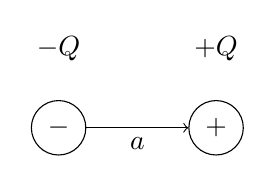
\begin{tikzpicture}
	\node[draw,circle] (qm) at (-1,0) {$-$};
	\node[above of=qm] {$-Q$};
	
	\node[draw,circle] (qp) at (1,0) {$+$};
	\node[above of=qp] {$+Q$};
	
	\draw[->] (qm) to (qp) node[midway, below] {$a$};
\end{tikzpicture}
\end{figure}

The electric dipole moment is
\begin{equation}
	\vec{p} = Q \vec{a}
\end{equation}

When placed in an external electric field $E$, an atom will develop an induced dipole moment
\begin{equation}
	\vec{p}_{\text{induced}} = \alpha \vec{E}
\end{equation}
where $\alpha$ is the electronic polarizability (also $\alpha_e$)

\subsection{Resonance frequency}
To achieve an equilibrium of displacement $x$, the force applied by the electric field $F_e = Ze E$ (where $Z$ is the number of electrons, thus $Z e$ is the displaced charge) has to be equal to the retracting force $F_r = -\beta x$.
Thus $x = \frac{Ze E}{\beta}$. 
The induced el. dipole moment is $p_e = (Ze) x = \frac{(Ze)^2 E}{\beta} = \alpha_e E$.

Assuming a harmonic motion, one finds the differential equation $(Z m_e) \ddot{x} = -\beta\dot{x}$ with the resonance frequency $\omega_0 = \sqrt{\frac{\beta}{Z m_e}}$.

The electronic polarization is then
\begin{equation}
	\alpha_e = \frac{Z^2 e^2}{\beta} = \frac{Z e^2 }{m_e \omega_0^2}
\end{equation}

and the resonance frequency is
\begin{equation}
	\omega_0 = 2 \pi f_0 = \left( \frac{\beta}{Zm_e} \right)^{1/2}
\end{equation}

\subsection{Polarization vector}
The polarization vector $\vec{P}$ is defined as the total dipole moment per unit volume
\begin{equation}
	\vec{P} = N \vec{p}_{av}
\end{equation}
where $N$ is the number of molecules per unit volume and $\vec{p}_{av}$ is the average dipole moment.

For a parallel plate capacitor it follows that
%TODO: add image maybe?
\begin{equation}
	P = \frac{p_{\text{total}}}{\text{volume}} = \frac{Q_P d}{A d} = \frac{Q_P}{A} = \sigma_P
\end{equation}
where$Q_P$ is the positive and negative surface charge ($\pm Q_P$) and $\sigma_P$ is the surface polarization charge density.

The electric susceptility $\chi_e$ is
\begin{equation}
	\chi _e = \frac{1}{\varepsilon_0} N \alpha_e
\end{equation}
From $\vec{D}=\varepsilon_0 \vec{E} + \vec{P} = \varepsilon_0\varepsilon_r \vec{E}$, it follows that
\begin{equation}
	\varepsilon_r  = 1 + \chi_e = 1 + \frac{N \alpha_e}{\varepsilon_0}
\end{equation}

\subsection{Clausius-Mosotti Equation}
The local field in dielectrics is given by
\begin{equation}
	E_{loc} = E + \frac{1}{3 \varepsilon_0} P
\end{equation}

As the local field $E_{loc}$ is larger than the applied field $E$, the Clausius-Mosotti equation is
\begin{equation}
	\frac{\varepsilon_r - 1}{\varepsilon_r+2} = \frac{N \alpha_e}{3 \varepsilon_0}
\end{equation}


\clearpage
\appendix
\section{Periodic table}
\begin{table}[ht!]
    \centering
    \includegraphics[height=0.9\linewidth,angle=90]{images/Periodic_Table.pdf}
    \caption{The periodic table of elements}
    \label{tab:app_periodictable}
\end{table}

\section{Seebeck coefficients}\label{app:Seebeck}
\begin{table}[ht!]
    \centering
    \begin{tabular}{lllll}
    Metal & S at \SI{0}{\degreeCelsius} (\si{\micro\volt\per\kelvin}) & S at \SI{27}{\degreeCelsius} (\si{\micro\volt\per\kelvin}) & $E_F$ (\si{\eV}) & x \\ \toprule
    Al   & -1.6    & -1.8   & 11.6 & 2.78    \\
    Au  & +1.79 & +1.94 & 5.5   & -1.48  \\
    Cu  & +1.70 & +1.84 & 7.0   & -1.79  \\
    K    &            &  -12.5 & 2.0   & 3.8      \\
    Li   & +14     &           & 4.7    & -9.7    \\
    Mg & -1.3    &           & 7.1    & 1.38     \\
    Na  &            & -5      & 3.1   & 2.2        \\
    Pd  & -9.00   & -9.99 &         &             \\
    Pt  & -4.45    & -5.28 &         &             \\ \bottomrule
    \end{tabular}
    \caption{Seebeck coefficients of selected materials. (Source: Kasap, Table 4.3)}
    \label{tab:app_seebeck}
\end{table}


\end{document}
